\section{Analytical details}
\label{app:analysis}

\subsection{Finite conditional response}

Let the product-state angle map be affine,
$\alpha(c)=b+Wc$, where row $i$ of $W$ is $w_i^{\mathsf T}$. Expanding each
local sine and cosine into exponentials shows that every amplitude has
frequencies in signed sums of the rows of $W$. Squaring an amplitude gives
\begin{equation}
 \Omega_{\mathrm{full}}(W)
 \subseteq
 \left\{\sum_{i=1}^{n}s_iw_i:s_i\in\{-1,0,1\}\right\}.
\end{equation}
Coincident frequencies and vanishing coefficients can make the inclusion
strict. The argument establishes a finite response space at fixed encoding
width; it does not provide an efficient coefficient-evaluation procedure or a
universal-approximation result.

For an observable $Z_a$, the active-generator expansion retains only
generators with $a\cdot g_j=1\pmod 2$. Grouping active subsets by their XOR
mask $h$ and using $\langle Y_i\rangle=0$ for a real $R_Y$ product input
removes terms with $h\wedge a\ne0$. Observable responses can therefore have
strictly smaller frequency support than full probabilities. This is a direct
specialization of established circuit-Fourier and IQP active-generator
descriptions
\cite{schuldEffectDataEncoding2021,casasMultidimensionalFourier2023,
recio-armengolTrainClassicalDeploy2026}.

\subsection{Product and block-product estimator}

Write the tractable reference amplitude as
$\phi_c(z)=\langle z|H^{\otimes n}|\phi(c)\rangle$. The classical
observable estimator samples $z$ from $|\phi_c(z)|^2$ and evaluates an
amplitude ratio $R_c(z,a)=\phi_c(z\oplus a)/\phi_c(z)$ together with the
phase factor generated by the active diagonal terms. The ratio obeys
\begin{align}
 \E_z|R_c(z,a)|^2
 &=\sum_{z:|\phi_c(z)|>0}|\phi_c(z)|^2
   \frac{|\phi_c(z\oplus a)|^2}{|\phi_c(z)|^2} \\
 &\leq \sum_z|\phi_c(z\oplus a)|^2=1.
\end{align}
The equality used in the main text holds when the shifted support is fully
covered; the inequality is the general statement when some reference
amplitudes vanish. In either case the variance is at most one. The bound is on
the estimator variance, not on optimizer convergence or raw gradient
magnitude.

The same argument applies to a block-product input
$|\phi(c)\rangle=\bigotimes_B|\phi_B(c)\rangle$. The ratio factorizes over
blocks, and normalization gives
\begin{equation}
 \E|R_c(z,a)|^2
 \leq\prod_B\sum_{z_B}|\phi_B(z_B\oplus a_B)|^2=1.
\end{equation}
This observation supports the archived block-encoding study in
Sec.~\ref{app:encoding}. The Gaussian production experiments use single-qubit
product states, while the Curie--Weiss production experiments use the
spin-flip two-branch state, whose radial amplitude also factorizes over
Hamming shells and is classically tractable.

\subsection{Hamming-kernel character loss}

For $a_i\sim\operatorname{Bernoulli}(q_\sigma)$ with $q_\sigma$ defined in
Eq.~\eqref{eq:mask-law},
\begin{align}
 \E_a[(-1)^{a\cdot(x\oplus y)}]
 &=\prod_i\bigl[(1-q_\sigma)+q_\sigma(-1)^{x_i\oplus y_i}\bigr]\\
 &=\exp[-d_H(x,y)/(2\sigma^2)].
\end{align}
For condition set $C$, the training objective is the balanced average
\begin{equation}
 \mathcal L(\theta)=\frac{1}{|C|}\sum_{c\in C}
 \mmd^2(q_\theta(\cdot\mid c),p(\cdot\mid c)).
\end{equation}
Independent model and target draws give the standard unbiased U-statistic.
All random streams for masks, model samples, target batches, and validation
are derived separately and recorded in the campaign artifacts.

\section{Gaussian protocol and complete factorial summary}
\label{app:gaussian-protocol}

For each $n$, width factor $s$, and condition $c$, the target shell law is a
truncated discrete Gaussian. Its untruncated location is calibrated so that
the truncated mean is exactly $n(0.15+0.70c)$, and its nominal width is
$s\sqrt n$. Conditional and no-condition models share the complete two-local
generator bank, initialization, datasets, optimizer seed, minibatches, and
estimator streams. Single-condition references use condition-tagged streams.

The factorial contains $4\times3\times10$ seed cells and 840 atomic fits.
The condition-count study adds 180 fits for a total of 1,020. Training uses
10,000 strings and validation uses 2,000 strings per condition in the
fixed-per-condition regime. The fixed-total regime divides 18,000 training and
3,600 validation strings across conditions using prefixes of the same master
pools. Held-out conditions have no sample role in the stored datasets.

Table~\ref{tab:factorial-all} reports every size--width profile-TVD effect.
Positive no-condition effects favor conditioning. Positive adjacent-reference
or mixture effects would favor the shared model.

\begin{table*}[t]
\centering
\scriptsize
\caption{Gaussian factorial profile-TVD effects with paired 95\% bootstrap
intervals. Status letters are S for supported, M for mixed, and U for
unsupported, in the order no-condition, adjacent-reference, mixture.}
\label{tab:factorial-all}
\begin{tabular}{@{}rrp{0.21\textwidth}p{0.21\textwidth}
  p{0.21\textwidth}l@{}}
\toprule
$n$ & $s$ & no condition $-$ conditioned &
adjacent reference $-$ conditioned &
mixture $-$ conditioned & status\\
\midrule
\tableinput{generated/factorial_cells.tex}
\bottomrule
\end{tabular}
\end{table*}

Table~\ref{tab:condition-count-compact} shows the condition-density result
used in the main text. The full per-condition rows, worst-condition values,
paired intervals, and exact probability vectors remain in the machine-readable
report.

\begin{table*}[t]
\centering
\small
\caption{Condition-count study at $n=19,s=0.50$. Mean and worst are held-out
profile TVD. The shared model keeps 190 phases and 2,000 updates.}
\label{tab:condition-count-compact}
\resizebox{\textwidth}{!}{%
\begin{tabular}{rlllrrrrr}
\toprule
$K$ & regime & train/condition & validation/condition & mean & worst &
phases & shared updates & reference updates\\
\midrule
\tableinput{generated/condition_count_cells.tex}
\bottomrule
\end{tabular}}
\end{table*}

Profile TVD intentionally quotients out within-shell variation. The exact
raw-bitstring report shows that low profile error does not imply a uniform law
inside each shell. We retain the raw probabilities and all secondary metrics in
the release artifacts rather than reproducing hundreds of diagnostic rows in
the PDF.

\section{Curie--Weiss protocol and results}
\label{app:curie-protocol}

For $s_i=2x_i-1$, $M=\sum_i s_i$, and $n=8$, the exact target is
\begin{equation}
 p_\beta(x)=Z_\beta^{-1}\exp\!\left(\frac{\beta M^2}{2n}\right).
\end{equation}
The campaign checks normalization, permutation invariance, and spin-flip
invariance before writing a dataset. Each of ten dataset archives contains
10,000 training and 2,000 validation strings at the six training
temperatures. Exact laws at held-out midpoints enter only after checkpoint
selection.

The v3 broadcast map is piecewise linear. Its knots were chosen from
development screens before production and are recorded in the manifest. The
map is not presented as target-independent. The production model uses the
spin-flip two-branch state on eight visible and five ancilla inputs, applies a
complete two-local 13-qubit IQP unitary, and sums the exact joint law over all
ancilla outcomes. The encoding family and map were frozen before the 80
production fits.

Table~\ref{tab:cw-effects} gives the complete aggregate comparison set.
Temperatures are averaged within seed before bootstrapping. Positive effects
favor the named conditioned model. The shared model matches the adjacent
mixture and improves on the target-aware adjacent oracle in this campaign;
both profile and raw TVD improve relative to no conditioning.

\begin{table*}[t]
\centering
\scriptsize
\caption{All paired Curie--Weiss v3 effects.}
\label{tab:cw-effects}
\begin{tabular}{p{0.62\textwidth}cc}
\toprule
comparison & effect [95\% interval] & status\\
\midrule
\curieweissancillaeffects
\bottomrule
\end{tabular}
\end{table*}

The five-ancilla choice followed a separate three-seed development study at
$r\in\{0,1,3\}$. It motivated adding latent capacity but did not test
$r=5$, establish an optimal ancilla count, or isolate mixed-state rank from
parameter count.

\begin{table}[t]
\centering
\caption{Ancilla development study. Entries are mean held-out TVD.}
\label{tab:cw-ancilla-pilot}
\begin{tabular}{rrcc}
\toprule
$r$ & model & profile TVD & raw TVD\\
\midrule
\curieweissancillapilot
\bottomrule
\end{tabular}
\end{table}

\subsection{Historical v2 matched-capacity diagnostic}

This diagnostic predates the v3 spin-flip campaign. It compares the v2
product-input ancilla model with a visible-only model containing every
nonempty one-, two-, and three-qubit diagonal generator on eight visible
qubits:
\begin{equation}
 \binom81+\binom82+\binom83=8+28+56=92.
\end{equation}
This is one phase more than the five-ancilla complete two-local model. The
control reuses the v2 datasets, product-input angle map, support-hashed
initialization, estimator streams, 2,000-step optimizer, validation checkpoint
rule, and exact evaluation grid. It does not reuse the v3 input state and is
therefore neither a capacity match for v3 nor evidence that ancillas cause the
v3 improvement. Critical aggregates average
$\beta\in\{0.9,1.0,1.1\}$; cold aggregates average
$\beta\in\{1.3,1.4,1.5\}$.

\ifcapacitycontrolresults
\begin{table}[t]
\centering
\caption{Matched-capacity paired effects. Positive values mean lower TVD for
the five-ancilla model.}
\label{tab:capacity-effects}
\begin{tabular}{lcc}
\toprule
region & profile TVD & raw TVD\\
\midrule
held out & \CapacityProfileHeldOut{} & \CapacityRawHeldOut{}\\
critical & \CapacityProfileCritical{} & \CapacityRawCritical{}\\
cold & \CapacityProfileCold{} & \CapacityRawCold{}\\
\bottomrule
\end{tabular}
\end{table}
\fi

\begin{figure}[H]
\centering
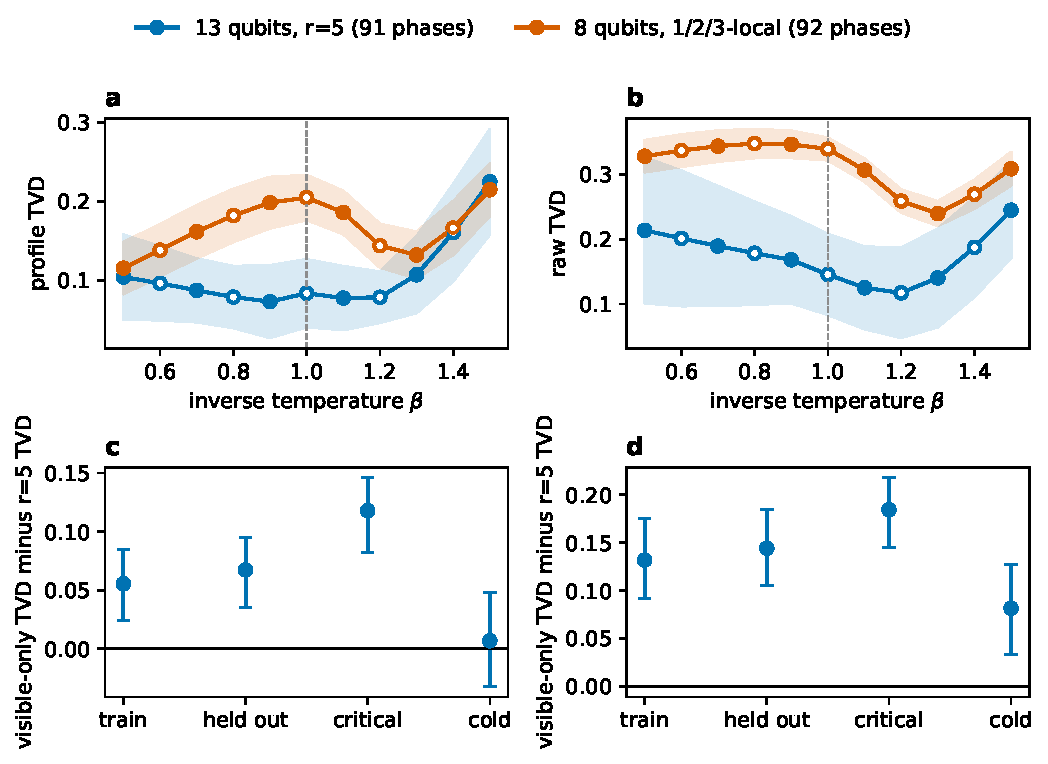
\includegraphics[width=\textwidth]{curie_weiss_ancilla_figures/matched_capacity_v2.pdf}
\caption{Historical v2 matched-capacity diagnostic. Mean profile and raw TVD
and paired regional effects compare the 91-phase v2 product-input ancilla
model with the 92-phase visible-only model. Positive effects favor the v2
ancilla model. This is not a matched control for the v3 spin-flip model.}
\label{fig:capacity-control}
\end{figure}

\section{Exploratory symmetry screens}
\label{app:symmetry-screens}

These post-core screens test whether matching an input state's symmetry to a
target can improve finite-system fits. They were designed after the core
campaigns and are not confirmatory evidence for the v3 result.

\paragraph{Two-block $Z_2^2$.} A two-block Curie--Weiss target
$p(s)\propto\exp[\beta(M_A^2+M_B^2)/16]$ on two eight-spin blocks is invariant
under independently flipping each block. The tested input is a product of two
two-branch states,
$|\phi\rangle=(|p_A\rangle^{\otimes8}+X^{\otimes8}|p_A\rangle^{\otimes8})
\otimes(|p_B\rangle^{\otimes8}+X^{\otimes8}|p_B\rangle^{\otimes8})$.
Across ten matched seeds it outperforms the product and single-$Z_2$ inputs on
the reported held-out metrics. This ordering is a screen result, not a general
theorem about symmetry-matched encodings.

\begin{figure}[H]
\centering
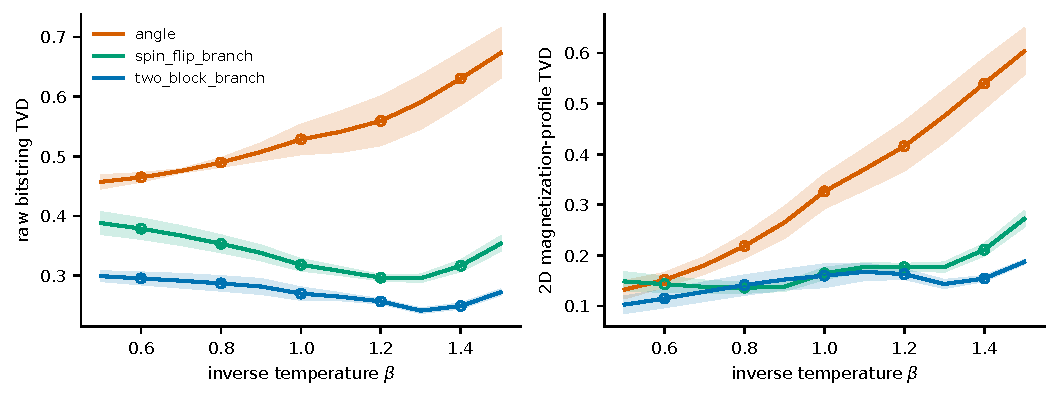
\includegraphics[width=\textwidth]{symmetry_figures/two_block_screen.pdf}
\caption{Exploratory two-block $Z_2^2$ screen. Held-out raw and two-block
magnetization-profile TVD for product, single-$Z_2$, and two-block-$Z_2^2$
inputs. Bands are one standard error across ten matched seeds; hollow markers
denote held-out temperatures.}
\label{fig:two-block}
\end{figure}

\paragraph{Asymmetric exchangeable targets.} A radial-shell state with a
frozen quartic shell law accepts two coordinates $(c_1,c_2)$ and preserves
permutation symmetry without enforcing spin flip. It improves the
weight-profile and permutation-averaged raw TVD in the reported screen, while
its unprocessed raw TVD is worse. The product and two-branch baselines receive
only $c_1$, whereas the radial model receives both $c_1$ and $c_2$; the result
therefore does not isolate symmetry matching from access to an additional
condition coordinate.

\begin{figure}[H]
\centering
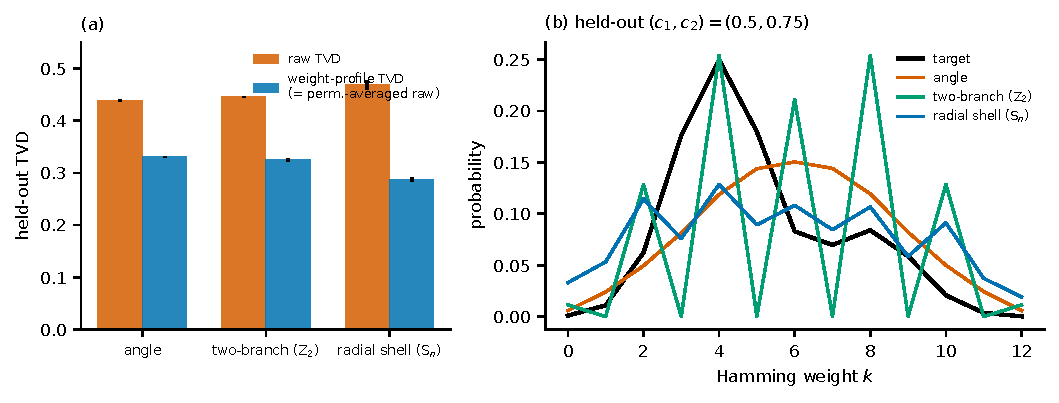
\includegraphics[width=\textwidth]{symmetry_figures/radial_shell.pdf}
\caption{Exploratory asymmetric radial-shell screen. Held-out raw and
weight-profile TVD and representative weight profiles are shown for the three
input families. The unequal condition information makes this a feasibility
screen rather than a controlled encoder comparison.}
\label{fig:radial}
\end{figure}

\section{Archived encoding comparison}
\label{app:encoding}

We tested two extensions of the single-angle product encoding on the
$n=19,s=0.50$ Gaussian task: noncommuting single-qubit reuploading and
two-qubit block-product inputs. None improved the tuned production encoder.
The study is supplementary because it followed a different development
protocol and its alternatives were not used in either production campaign.

\begin{table}[H]
\centering
\caption{Archived matched encoding comparison on the $n=19,s=0.50$
Gaussian task. Lower is better. The paired profile effect is relative to the
single-angle baseline; positive values are worse.}
\label{tab:encoding_benchmark}
\resizebox{\textwidth}{!}{%
\begin{tabular}{lcccc}
\toprule
encoding & structure & held-out profile TVD & held-out raw TVD & paired profile effect\\
\midrule
single angle & $L=1$ & $0.062\pm0.004$ & $0.348\pm0.006$ & baseline\\
noncommuting & $L=2$ & $0.072\pm0.009$ & $0.374\pm0.027$ & $+0.011$ [$+0.004,+0.017$]\\
block $ZZ$ & $\kappa=\pi/8$ & $0.070\pm0.008$ & $0.371\pm0.020$ & $+0.009$ [$+0.003,+0.015$]\\
block $ZZ$ & $\kappa=\pi/4$ & $0.071\pm0.014$ & $0.398\pm0.009$ & $+0.009$ [$-0.001,+0.017$]\\
\bottomrule
\end{tabular}}
\end{table}

\begin{figure}[H]
\centering
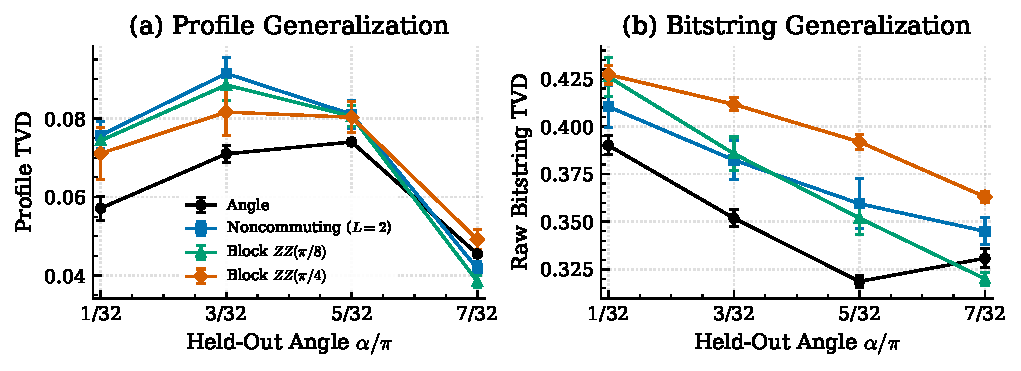
\includegraphics[width=\textwidth]{figures/encoding_benchmark.pdf}
\caption{Archived input-encoding comparison. The left panel reports held-out
conditional MMD and the right panel reports raw profile TVD for the four tested
architectures. Lower is better.}
\label{fig:encoding-benchmark}
\end{figure}

\section{Finite estimator audit}
\label{app:estimator-audit}

The separate estimator audit contains 21 deterministic synthetic cases over
qubit count, generator count, condition count, and condition dimension. It
uses bounded-degree and complete two-local generator families at $n=4$ and
$n=8$. Exact references are used where feasible; larger cases compare repeated
estimator draws. The audit records expectation and gradient-estimator errors,
runtime, memory, seeds, and content digests.

This is finite consistency and resource evidence only. It does not support an
asymptotic scaling claim, a statement about raw gradient magnitude, convergence
of the optimizer, or absence of barren plateaus. No full training run is
charged to this audit.

\section{Negative and boundary studies}

An eight-qubit pilot attempted joint conditioning on Gaussian location and
width. Its frozen design required adequate single-condition representability
before interpreting shared-model performance. Two narrow-width cells failed
that screen, so the study stopped. It supplies no evidence for
two-coordinate conditional generation and is retained as a negative result.

Older topology and ancilla studies remain archived under their original
protocols. They are not pooled with either production campaign. The two
symmetry screens above are supplementary exploratory evidence. Permutation
twirling is included only as target-symmetry-aware post-processing; it is not
a symmetry learned by the circuit.

\section{Campaign integrity and reproduction}
\label{app:reproduction}

The Gaussian and Curie--Weiss stores bind every run identity to a manifest,
role-tagged dataset, estimator streams, source digest, environment, code
revision, checkpoint, exact probability archive, invocation, runtime, and peak
memory. Stores reject undeclared identities, duplicate completion, and silent
reuse of partial results. Report, claim, table, and figure generators require
complete campaign state.

The Gaussian dependency closure includes a content-addressed snapshot of the
historical execution source. In particular, the archived
\texttt{encoding.py} has SHA-256
\texttt{0ec0d9d2903fd44684841721c9ffac9543f2c7f883e28f8ada09bb318e258338}.
The current live encoder is not substituted for that historical source.

The principal local reproduction commands are:
\begin{verbatim}
uv sync --frozen
uv run pytest -q
uv run ruff check src scripts tests
uv run python scripts/audit_gaussian_release.py
uv run python scripts/audit_curie_weiss_ancilla_release.py
uv run python scripts/run_curie_weiss_capacity_control.py run
uv run python scripts/run_curie_weiss_capacity_control.py summarize
(cd paper && latexmk -pdf main.tex)
\end{verbatim}

Exhaustive per-seed and per-condition tables remain in JSON, NPZ, and generated
TeX artifacts in the local review package. Keeping them machine-readable
preserves the audit trail without turning the supplement into a second report.
